{\let\clearpage\relax \chapter{Evaluation}\label{ch:eval}}
In this section, we evaluate the performance of literature search queries based on the introduced metrics. This evaluation serves as a foundation for developing tools that can potentially generate automatic literature search queries in the future. It is crucial to note that the objective of this evaluation is not only to assess the SQW tool itself but also to show how the defined metrics affect any arbitrarily generated literature search query. This allows us to evaluate the quality of the query regardless of the method by which it was generated.

\vspace*{.5cm}

\section{Experimental Setup}
The curated dataset is constructed using two distinct methods to identify core publications: Bibliometric Analysis (14 topics) and Systematic Literature Review (7 topics), as illustrated in \autoref{fig:dataset-overview}. For the SLRs, the original queries used by the researchers are available. Consequently, we conduct two main experiments. In both experiments we use Dimensions.ai to retrieve all required data. The retrieval process relies on their default relevance-based sorting method, which ranks publications based on the number of keyword matches between the title-abstract and the provided query.

The first experiment involves all 21 topics from both the SLRs and BAs, where we compare a baseline query against a query generated by the SQW. The baseline query consists of the exact topic name, passed into the search engine in a non-exact fashion. For instance, the query \textit{Soft Robotics} retrieves publications containing both words in their title or abstract, even if they do not appear consecutively. 

The predicted query, however, is semi-automatically generated using the SQW tool. This process begins by providing the baseline query as input, which generates a list of keywords. These keywords are then manually sorted by the author into specific or general categories, as described in \autoref{fig:sqw-stage1}. The overarching topic is derived from the topic itself; for example, in the case of \textit{Soft Robotics}, the overarching keyword \textit{Robot} is used. In some cases, the resulting queries produced excessively large results (>100k publications). To address this, keywords were filtered to limit the results to a maximum of 50k publications, balancing evaluation cost and processing speed. Importantly, the baseline query is always included in the predicted query. This ensures that recall is at least as high for the predicted query as for the baseline, making the primary goal of the evaluation to determine whether the expanded query retrieves more core publications than the baseline without becoming overly general by retrieving irrelevant publications.

The second experiment focuses exclusively on the 7 SLR topics. It uses the exact baseline queries and results from the first experiment but compares them to SLR queries manually crafted by experts in the field rather than those generated by the SQW. These SLR queries are designed with well-defined research questions aimed at retrieving the most relevant publications that help tackle these exact questions.

\section{Results}
Using the data from the first experiment, we computed all the metrics, namely: Cosine Precision, Clustering Precision, MVEE Precision, Hull Precision, Recall, and the F2 score for each precision metric, as shown in \autoref{fig:all-metrics-1}. When examining the precision metrics, Clustering Precision distinctly stands out due to its high value in certain cases when evaluated on the predicted query. For example, both \textit{Software Fault Prediction Metrics} and \textit{Multicore Performance Prediction} achieve a clustering precision of 1.0, which happens because we cannot segment the large cluster into smaller ones while maintaining the threshold of required CPs, meaning that the smallest possible cluster is in fact the full space.

Low recall can also be an issue when computing Hull, MVEE, and Clustering Precision. For example, this issue is evident in the baseline evaluation for \textit{Multicore Performance Prediction}, \textit{Nanopharmaceuticals OR Nanonutraceuticals}, \textit{Sustainable Biofuel Economy}, \textit{Drones in Agriculture}, and \textit{Resilience in Business and Management}. The precision value for MVEE and Hull are both set to 0 manually, because the minimum required points to define a plane is 3, which are not available in this case. For clustering, it is also set to 0 due to two reasons: 1) The condition $\text{CPs} < 2$ that is defined in \autoref{algo:sp-clustering},
2) The threshold $\theta = 0.7$, which means that we need at least 4 CPs in order to be able to perform the algorithm, because $ \theta * 2 = 1.4 $ and $ \theta * 3 = 2.1 $.

\begin{figure}[!h]
	\hspace*{-1cm}	
	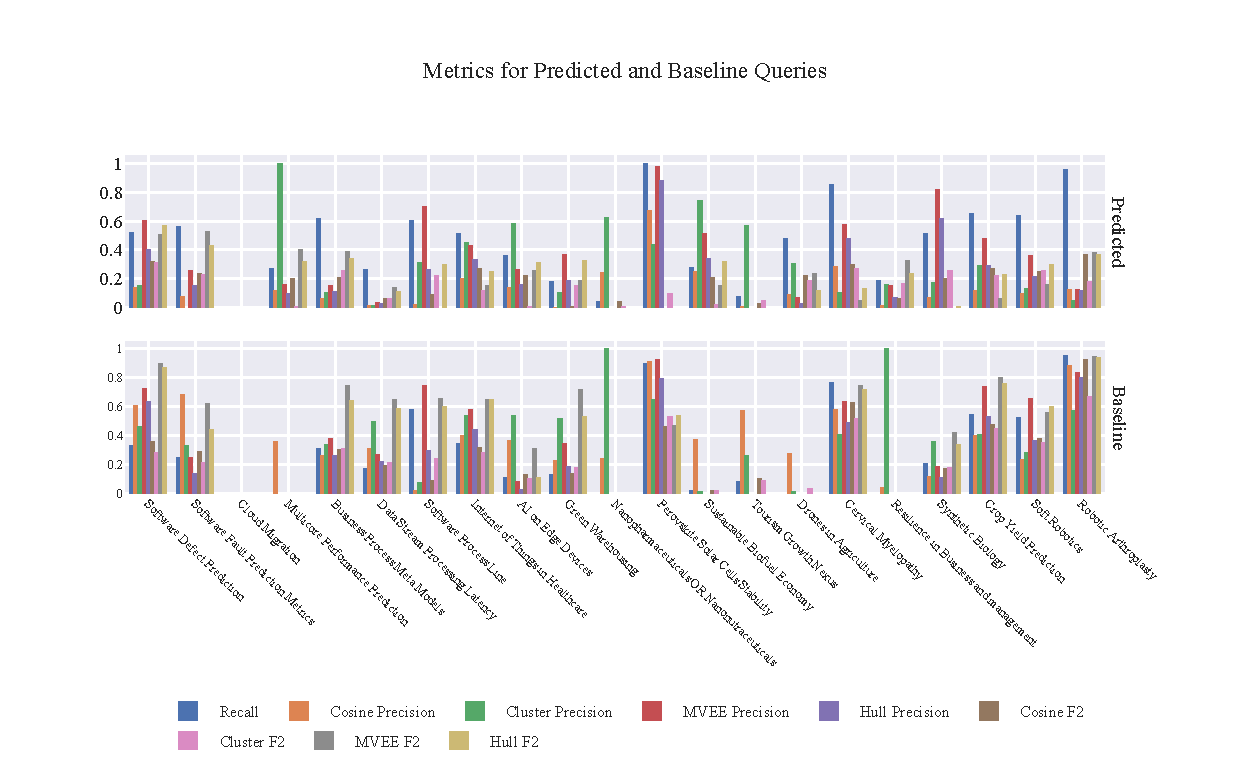
\includegraphics[scale=0.45]{pics/all-metrics-1.pdf}
	\caption[Evaluation: Experiment 1]{This figure shows the results of the first experiment across the datasets. An issue of the MVEE, and Hull precision metrics becomes apparent in baseline query for \textit{Drones in Agriculture} and \textit{Multicore Performance Prediction}, where the value is 0. This occurs because the retrieved CPs are $<3$, which is minimum number of CPs required to define a plane. Additionally, the impact of the decay parameter is particularly evident in cases like \textit{Robotic Arthroplasty}, where the baseline F2 score is very high. Conversely, for the predicted query, which retrieves more publications but maintains the same recall, the score is significantly lower.}\label{fig:all-metrics-1}
\end{figure}

In \autoref{fig:eval1_results}, we can better interpret the results of the first experiment by examining the differences between the scores of the predicted query and the baseline. Here, positive values indicate that the predicted query performs better, while negative values show that the baseline outperforms the predicted query. 

Considering the F2 score, a notable example of the impact of overly large queries without any recall improvement is \textit{Robotic Arthroplasty}. Both the baseline and predicted queries achieved a recall of 0.957, but the expanded predicted query from the SQW retrieved significantly more results overall. Specifically, the predicted query retrieved 22,892 publications, of which only 2,834 were relevant based on cosine similarity. In contrast, the baseline query retrieved 2,151 publications, with 1,904 classified as relevant. This demonstrates how an excessively large query can dilute the precision by increasing the total number of relevant documents retrieved without improving recall.

\begin{figure}[!t]
	\hspace*{-.8cm}	
	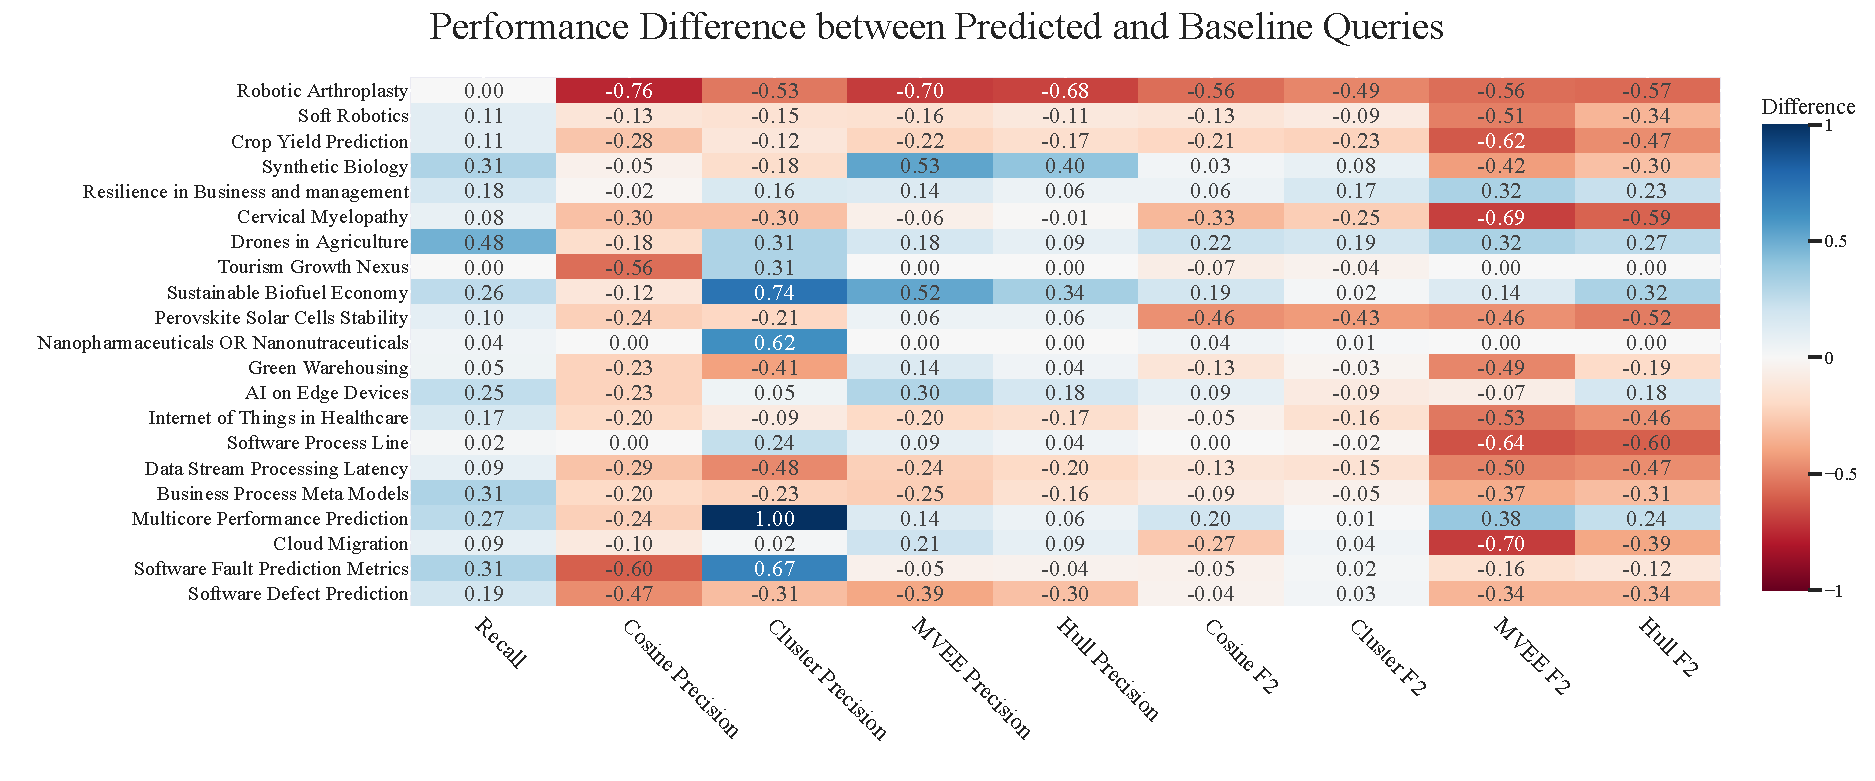
\includegraphics[scale=0.45]{pics/eval1_results.pdf}
	\caption[Evaluation Difference: Experiment 1]{In this figure we can see the difference in values between the predicted query from the SQW and the baseline, whereby a negative value means that the baseline is better. As anticipated we at least always achieve a similar recall, but in most cases, the SQW yields better recall. However, it severely suffers in precision. When looking at the F2 value, we can see that the tool only notably outperforms the baseline on the three topics \textit{Drones in Agriculture}, \textit{Sustainable Bio Fuel Economy}, and \textit{Multicore Performance Prediction}, whereas it shows a clear disadvantage on the topics \textit{Perovskite Solar Cells Stability}, \textit{Robotic Arthroplasty}, and \textit{Cervical Myelopathy}.}
	\label{fig:eval1_results}
\end{figure}

The results of the second experiment, which compares the actual search queries used to identify the core publications in the SLRs, are shown in \autoref{fig:all-metrics-2}. Overall, the results between the two approaches are comparable. However, the SLR queries were reconstructed to fit Dimensions' query criteria and the output format of the SQW, which have led to a degradation in their quality. Notably, the field of \textit{Multicore Performance Prediction} stands out, as it has a recall of 0 for both the SLR and baseline queries. In the case of the SLR query, this is due to the fact that only the initial query, without term expansion, was accessible \autocite{Frank2017}. The raw results for the baseline, predicted, and SLR queries can respectively be found in the appendix: \autoref{fig:baseline-results}, \autoref{fig:predicted-results}, and \autoref{fig:slr-results}.  

\begin{figure}[!t]
	\hspace*{-.8cm}		
	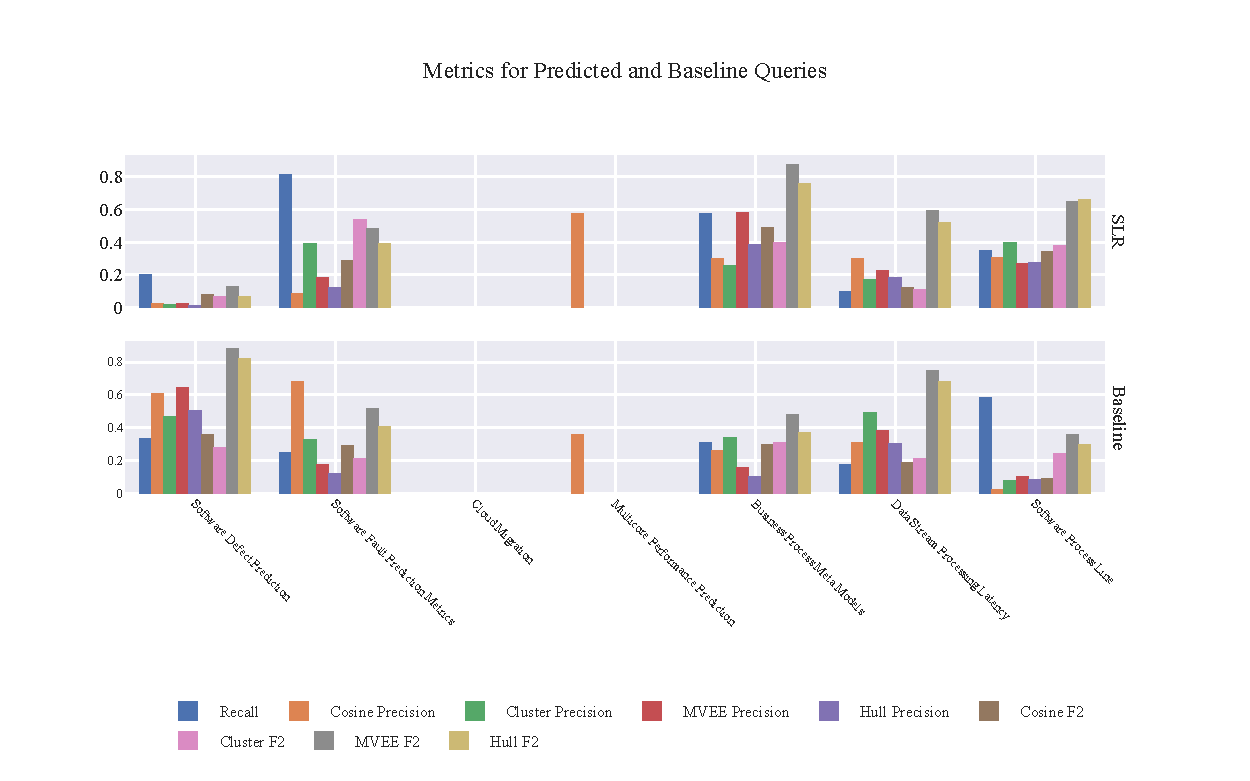
\includegraphics[scale=0.45]{pics/all-metrics-2.pdf}
	\caption[Evaluation: Experiment 2]{This figure shows the results of the second experiment across all the SLR datasets. Surprisingly, we can see that using the SLR query does not achieve outstanding results, which is attributed to its reconstruction and adaptation to fit dimension's search engine. Notably, the SLR query used for \textit{Multicore Performance Prediction} is only partially available for public access \autocite{Frank2017}, hence the very low scores.}\label{fig:all-metrics-2}
\end{figure}

In cases where the recall of the baseline significantly outperformed the SLR, namely \textit{Software Fault Prediction Metrics}, the cosine precision was much lower. This happened due to the unwanted behavior which can be interpreted by the cosine-F2 score being 0, indicating that the recall gain was of no value due to the excessive number of irrelevant retrieved publications.

In \autoref{fig:metrics-correlation} we observe the correlation between the metrics which ultimately showing us when to use which metric. The two important values to look at are the correlation between a precision metric with the recall, as well as their respective F2 score. For example, the Cosine precision poorly correlates with the recall, which means that more CPs will further lower the acceptance of publications as relevant, yet the correlation between the Cosine F2 and precision is decent, which means that sample is no too large to be negatively effected by the decay parameter. This suggests that the more CPs we have the more robust our cosine precision metric is.

\begin{figure}[!h]	
	\centering
	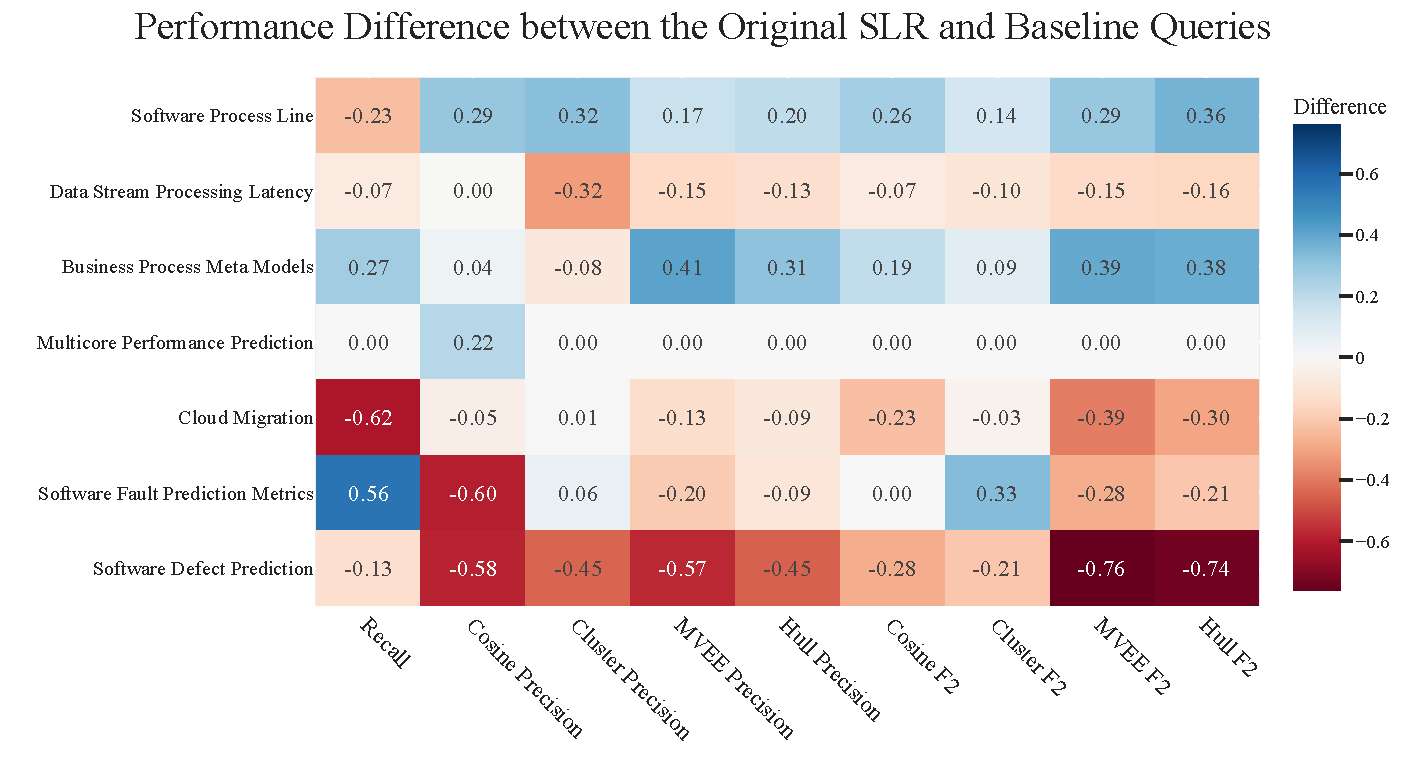
\includegraphics[scale=0.45]{pics/eval2_results.pdf}
	\caption[Evaluation Difference: Experiment 2]{This figure displays the metric values difference between the original SLR query and the baseline, where a negative value indicates that the baseline performs better. Overall, both queries show similar performance, with a few notable exceptions: in \textit{Cloud Migration}, the baseline query achieves significantly higher recall, whereas in \textit{Software Fault Prediction Metrics}, the SLR query has a much higher recall. In the case of \textit{Software Defect Prediction}, although the baseline query has a slightly better recall, it also demonstrates higher precision and a better F2 score, suggesting that it retrieves more relevant publications while maintaining low sample size.}
	\label{fig:eval2_results}
\end{figure}

\begin{figure}[!h]
	\centering
	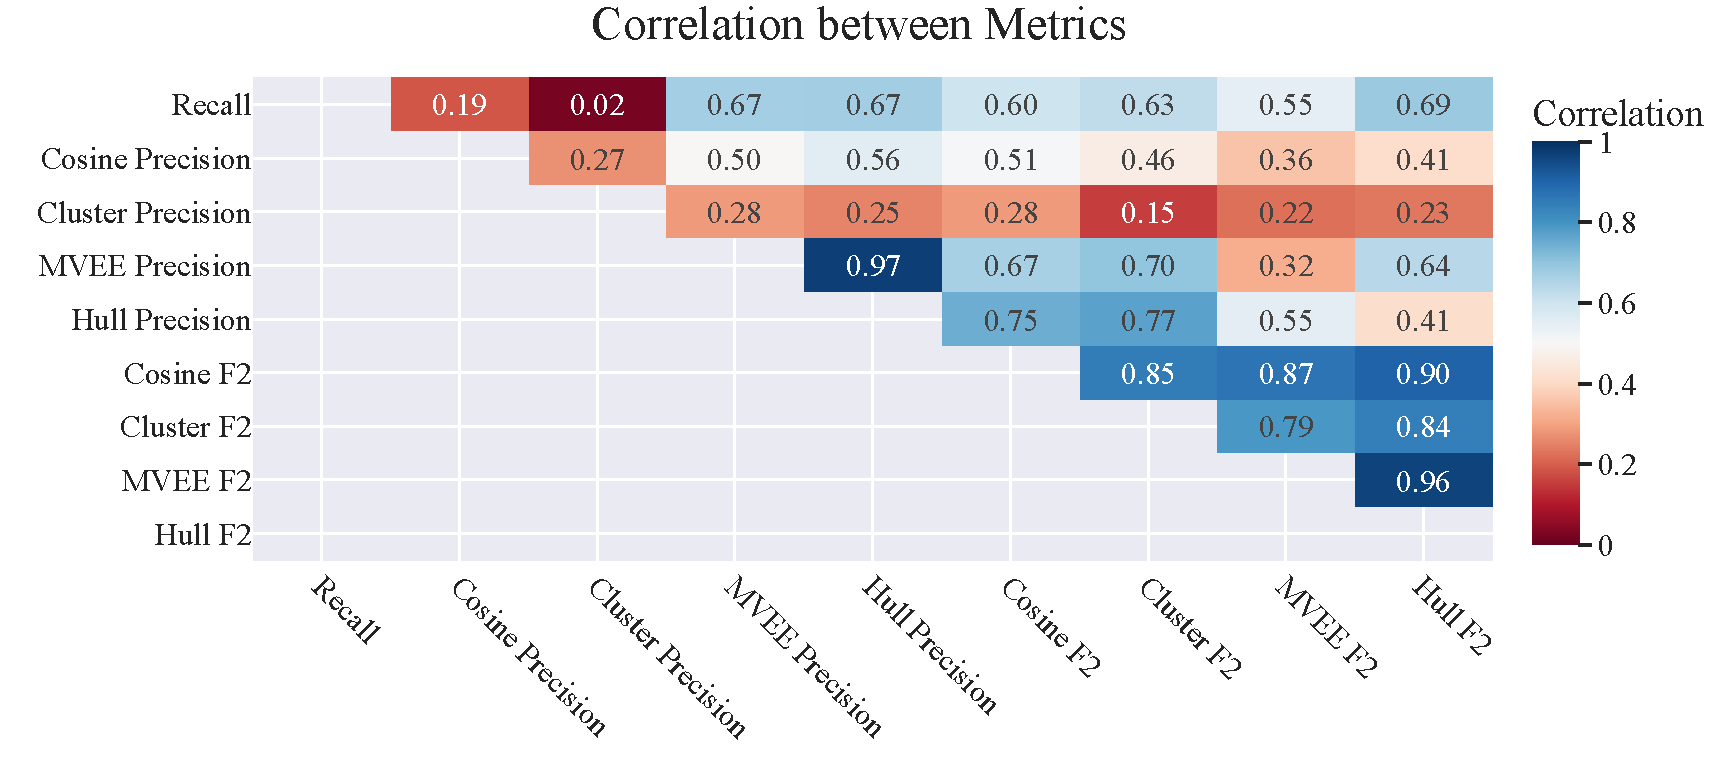
\includegraphics[scale=0.4]{pics/metrics_correlation.pdf}
	\caption[Metrics Correlation]{This figure shows the correlation between the various presented metrics. The cosine precision does not correlate well with recall, which indicates that higher recall corresponds to a robust precision metric, thereby affecting the cosine F2 score. In contrast, the Hull and MVEE precision metrics show strong correlation with recall, meaning that the number of relevant publications increases with recall, which has a negative impact their F2 scores. Clustering metrics appear to be unstable, showing no clear correlation with other factors.}
	\label{fig:metrics-correlation}
\end{figure}


In contrast Hull and MVEE precision seem to be the exact opposite, meaning that the more CPs we have the more publications we accept as relevant, which should increase their respective F2 score due to the higher precision value, but seems to negatively effect it, due to the decay factor increasing along the precision. The clustering precision there seems to be unpredictable thus the correlation between any of the other parameters is relatively low.

\section{Discussion}

The primary goal of this work was to determine the quality of literature search queries, emphasizing recall, which is widely regarded as an essential measure in the research community. However, precision has historically been less emphasized due to the intrinsic nature of literature search queries, which tend to favor comprehensiveness over specificity. By developing multiple metrics to evaluate the relevance of publications in a semantic space, we successfully integrated precision into the evaluation framework by introducing semantic precision.

To calculate semantic precision, we employed four metrics: semantic Cosine, Clustering, MVEE, and Hull precision. Each metric demonstrated distinct advantages and limitations. Initially, we hypothesized that the cosine similarity threshold should correspond to the least similar core publication. However, in certain cases, sacrificing a core publication to substantially reduce the number of irrelevant publications proved more beneficial in terms of the F2 score. Consequently, we adopted an empirical threshold estimated by maximizing the F2 score across all topics.

For Convex Hull and MVEE, we first tested their performance using the original embeddings in their high-dimensional space. However, these metrics consistently overestimated precision, often exceeding 50\%. This discrepancy is likely due to the curse of dimensionality, which complicates the construction of accurate ellipsoids or hulls in high-dimensional spaces, possibly reflecting limitations in the embedding construction process. This observation led to the decision to switch to UMAP embeddings, which offer a reduced dimensionality and improved computational feasibility. However, while UMAP embeddings show potential, the exact amount of semantic value lost compared to the original high-dimensional embeddings remains unclear.

The first experiment is as expected, the predicted query consistently achieves similar or better recall across all topics due to the inherent nature of the SQW. However, when evaluating precision, it is evident that the broader queries generated through query expansion often degrade the performance of the query. This effect is particularly visible in the F2 scores, where the increased number of irrelevant publications impacts the balance between recall and precision. While the SQW demonstrates advantages in terms of recall, its over-expansion often leads to noisy queries.

The results of the second experiment, shown in \autoref{fig:all-metrics-2}, which compare the actual search queries used to identify core publications in the SLRs, did not align with expectations, particularly in terms of recall, which was anticipated to be high. This discrepancy can be attributed to differences in how the queries were applied. The original SLR queries were designed for mixed search indices, including titles, abstracts, full text, and, in some cases, for specific fields and journals. However, for the results of this experiment to be comparable with the first experiment, the queries were adapted to fit output format of the SQW, which only produces keywords without any additional filtering. This adaptation effectively limited the scope of retrieval, making the results inherently dependent on the search engine used, in this case, Dimensions.ai.

A common issue for the Clustering, MVEE, and Hull methods lies in their dependency on recall. Semantic clustering requires at least 2 CPs for $\theta=0.5$, while this number increases depending on the value of $\theta$. Similarly, MVEE and Hull methods require at least 3 core publications to construct a plane that encloses other potentially relevant publications. In contrast, cosine similarity only requires the pre-computed mean embedding of the core publications and a similarity threshold. This independence from recall allows cosine similarity to determine relevance even when recall of the retrieved publications minimal, making it a more robust metric in cases of bad queries that retrieve no CPs.

Additionally, based on the impact of semantic precision and recall on the F2 score, as shown in \autoref{fig:metrics-correlation}, the most suitable precision should be the \textbf{Cosine Precision}. The reason is that it becomes more robust as the number CPs increases. However, for cases where the number of CPs is between 3 and 10, the Convex Hull precision could also be useful, as the number of relevant publications remains low enough to prevent significant impact on their F2 scores.





